\documentclass{article}
\usepackage[utf8]{inputenc}
\usepackage{titling}
\usepackage{graphicx}
\usepackage{xcolor}
\usepackage[colorlinks=true,linkcolor=darkgray, urlcolor =gray]{hyperref}
\usepackage[spanish]{babel}
\DeclareUnicodeCharacter{301}{~}
\usepackage{url}
\DeclareUnicodeCharacter{202F}{\,}


\title{Práctica WLAN: Parte 2}
\author{Cristina Díaz García}
\date{Diciembre 2018}

\renewcommand\maketitlehooka{\null\mbox{}\vfill}
\renewcommand\maketitlehookd{\vfill\null}


\begin{document}

\addcontentsline{toc}{section}{Índice general}

\begin{titlingpage}
\maketitle

\begin{center}

\includegraphics[scale=0.4]{WLAN/wireshark.jpg} 
\end{center}

\end{titlingpage}

\newpage

\tableofcontents

\newpage

\section{Cuestión 1}

\subsection{WLAN\_802\_11}

\textbf{¿Cuántas APs están en la cobertura de la estación desde la que se realizó la captura?}

Usando el filtro \textit{wlan.fc.type\_subtype == 0x0008} obtenemos las tramas Beacon. Guardamos los paquetes obtenidos como CSV, y haciendo uso del comando cut, obtenemos de la información el campo de los SSIDs. En total hay 4 APs.

\begin{center}
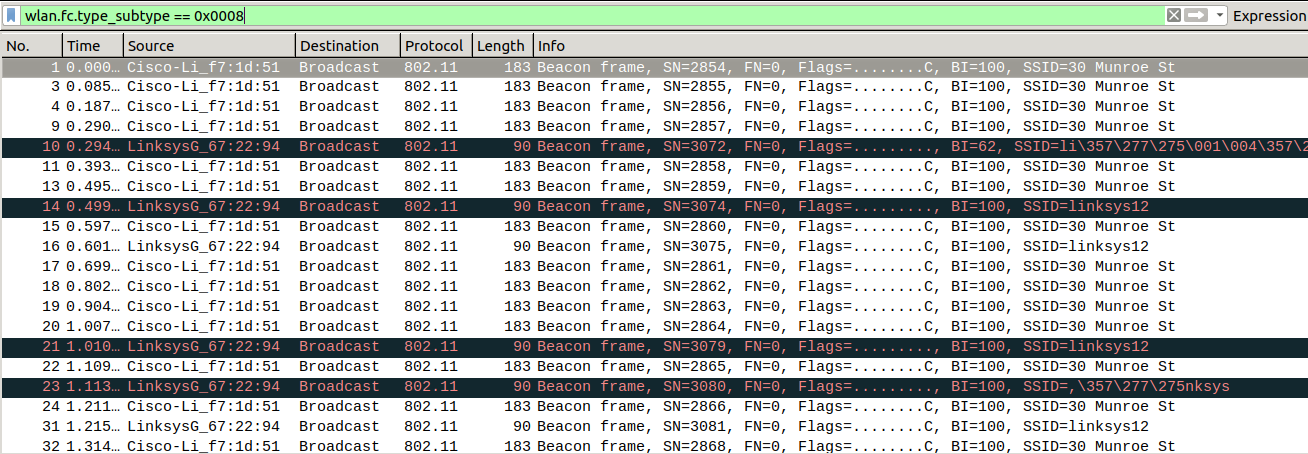
\includegraphics[scale=0.3]{WLAN/SSIDs.png}
\end{center}

\textbf{¿Cuales son sus identificadores?}

\begin{itemize}
\item 30 Munroe St
\item linksys12
\item linksys1R
\item linksys\_SES\_24086
\end{itemize}

Como se puede comprobar en la imagen siguiente, los nombres de los SSIDs están corruptos en algunos paquetes.

\begin{center}
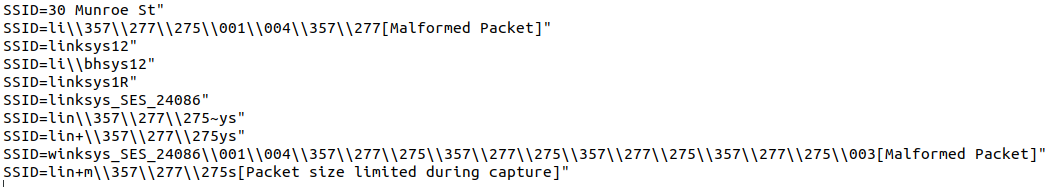
\includegraphics[scale=0.4]{WLAN/SSIDfinal.png}
\end{center}

\textbf{¿Cada cuanto tiempo envían una trama de Beacon?}

Cada décima de segundo aproximadamente.

\begin{center}

\includegraphics[scale=0.4]{WLAN/interval.png}
\end{center}

\textbf{¿Qué tipo de trama es? (valor de campo tipo)}

Es de tipo 0.

\begin{center}
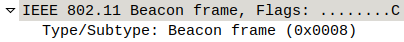
\includegraphics[scale=0.4]{WLAN/subtype.png}
\end{center}

\subsection{WLAN\_802\_11\_LOCAL}

\textbf{¿Cuántas APs están en la cobertura de la estación desde la que se realizó la captura?}

Usando el filtro \textit{wlan.fc.type\_subtype == 0x0008} obtenemos las tramas Beacon. Guardamos los paquetes obtenidos como CSV, y haciendo uso del comando cut, obtenemos de la información el campo de los SSIDs. En total hay 4 APs.

\begin{center}
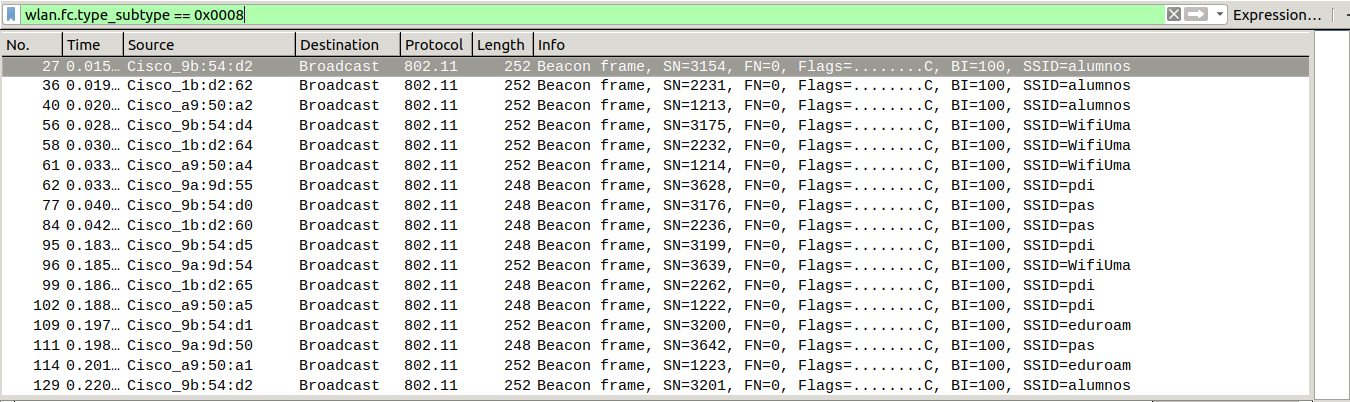
\includegraphics[scale=0.3]{WLAN/beacon.png}
\end{center}

\textbf{¿Cuales son sus identificadores?}

\begin{itemize}
\item alumnos
\item WifiUma
\item pdi
\item pas
\item eduroam
\item NEO
\item GISUM\_W1
\item ICB\-Wifi
\end{itemize}

\begin{center}
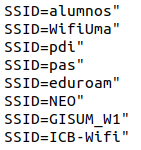
\includegraphics[scale=0.4]{WLAN/SSIDssss.png}
\end{center}

\textbf{¿Cada cuanto tiempo envían una trama de Beacon?}

Cada décima de segundo aproximadamente.

\begin{center}

\includegraphics[scale=0.4]{WLAN/interval.png}
\end{center}


\textbf{¿Qué tipo de trama es? (valor de campo tipo)}

Es de tipo 0.

\begin{center}
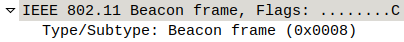
\includegraphics[scale=0.4]{WLAN/subtype.png}
\end{center}

\section{Ejercicio 1}

\textbf{Muestra la estructura y contenido de los campos de una trama Beacon (de ambos
ficheros)}

Al ser la estructura y el contenido de los campos el mismo, muestro una trama Beacon correcta y una corrupta del archivo \textit{WLAN\_802\_11}

\textbf{Trama Beacon correcta}

\begin{center}
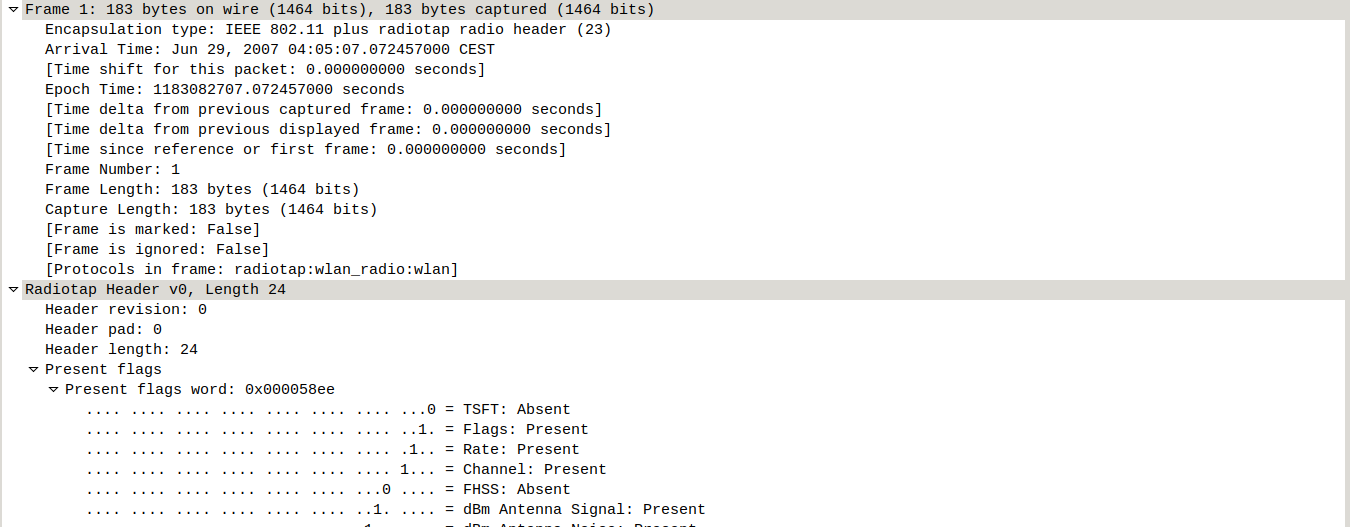
\includegraphics[scale=0.3]{WLAN/correcto1.png}
\end{center}
\begin{center}
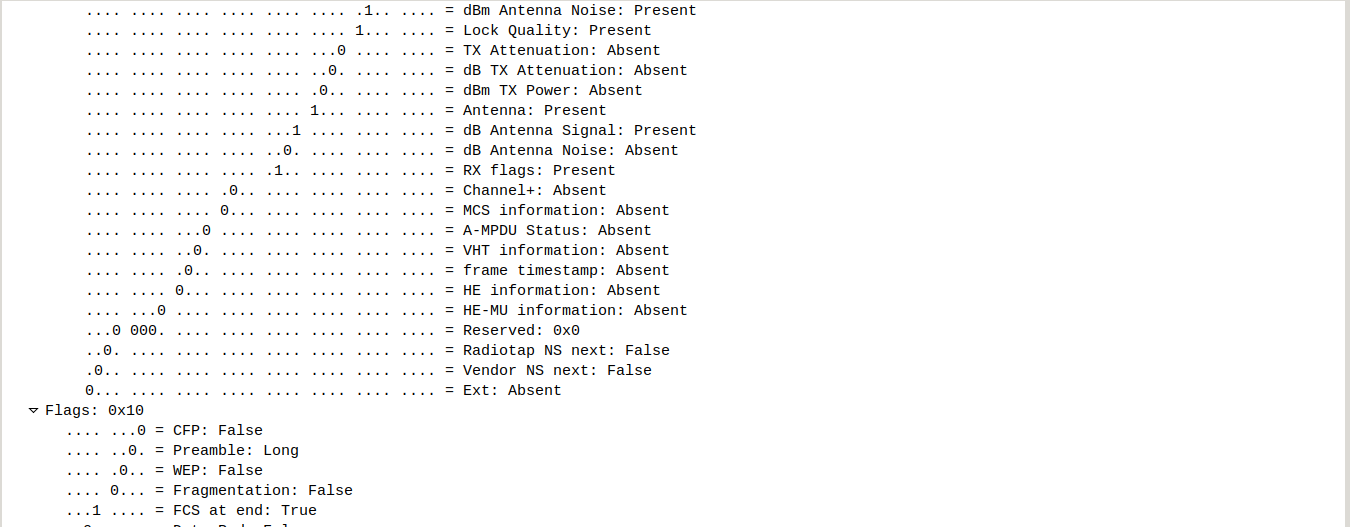
\includegraphics[scale=0.3]{WLAN/correcto2.png}
\end{center}
\begin{center}
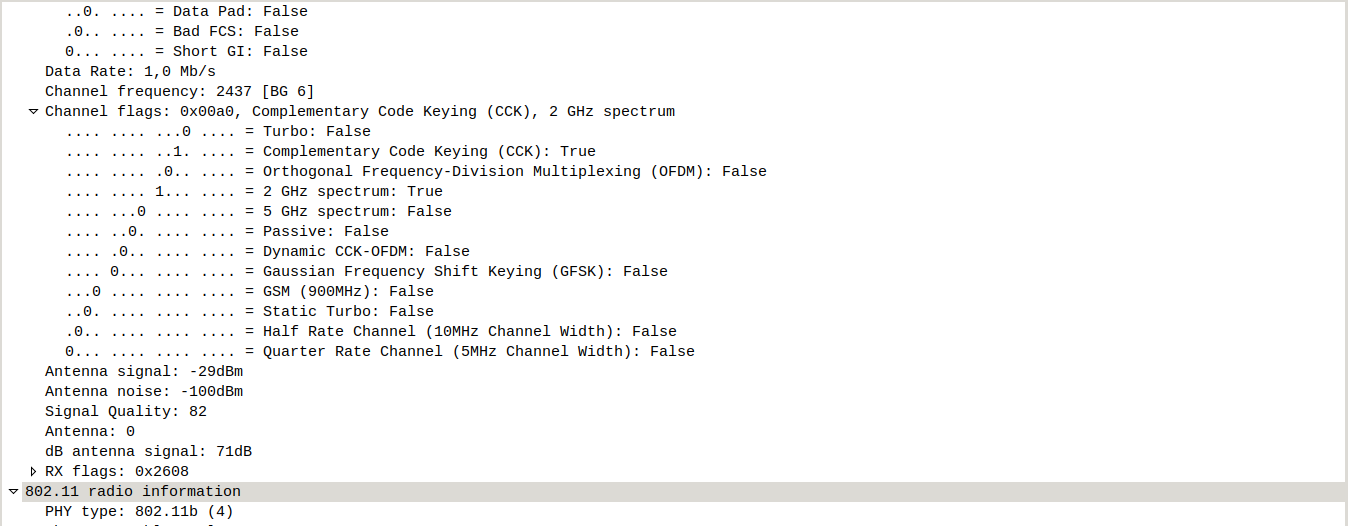
\includegraphics[scale=0.3]{WLAN/correcto3.png}
\end{center}
\begin{center}
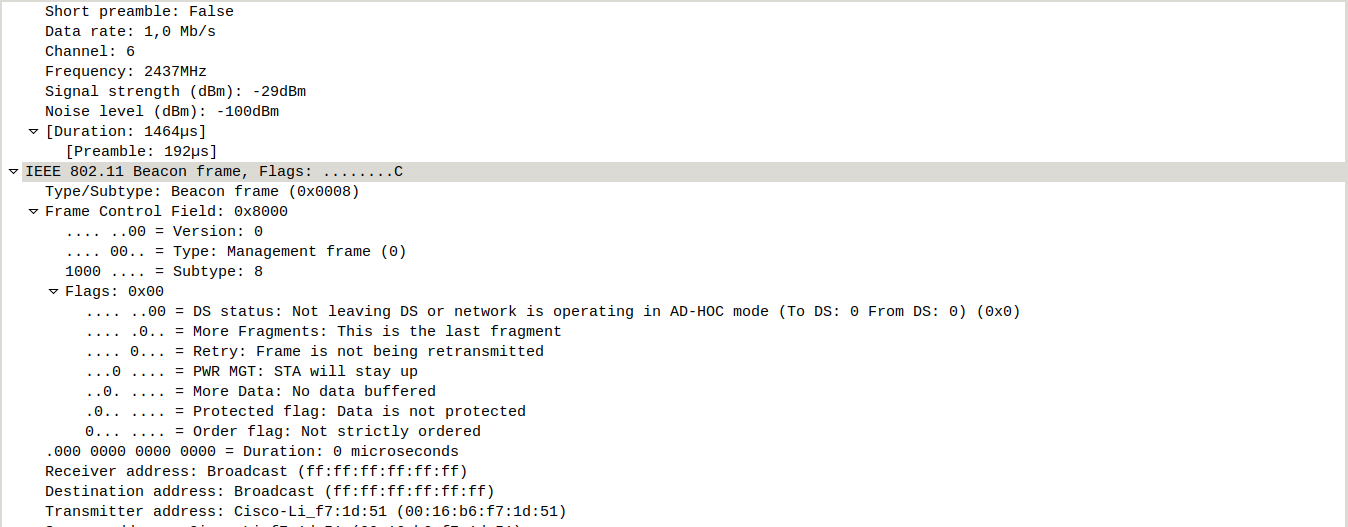
\includegraphics[scale=0.3]{WLAN/correcto4.png}
\end{center}
\begin{center}
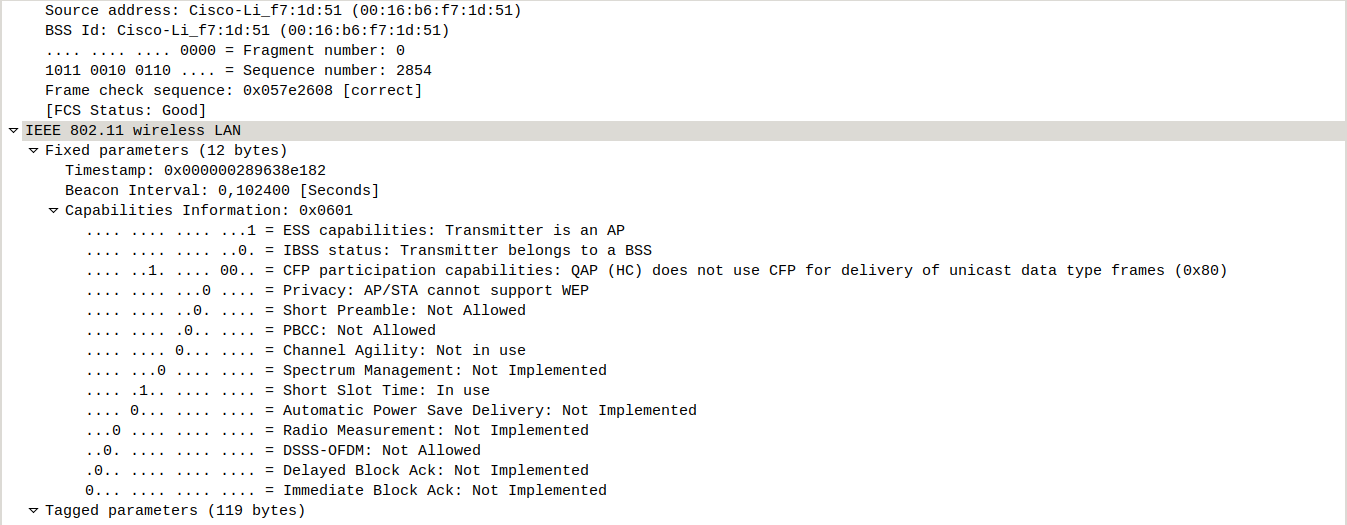
\includegraphics[scale=0.3]{WLAN/correcto5.png}
\end{center}
\begin{center}
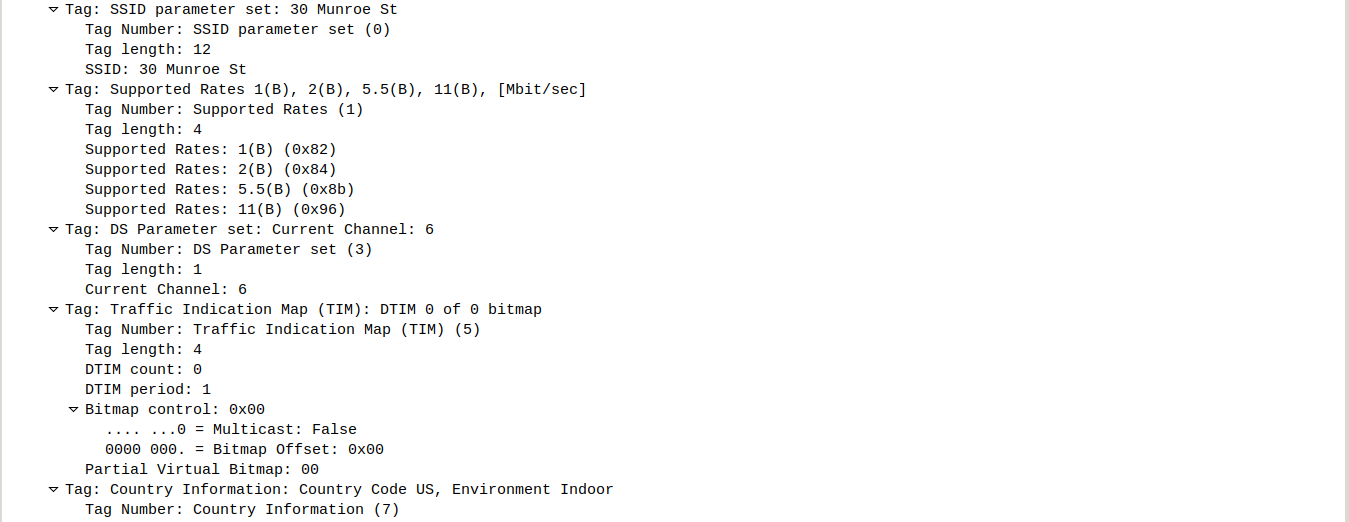
\includegraphics[scale=0.3]{WLAN/correcto6.png}
\end{center}
\begin{center}
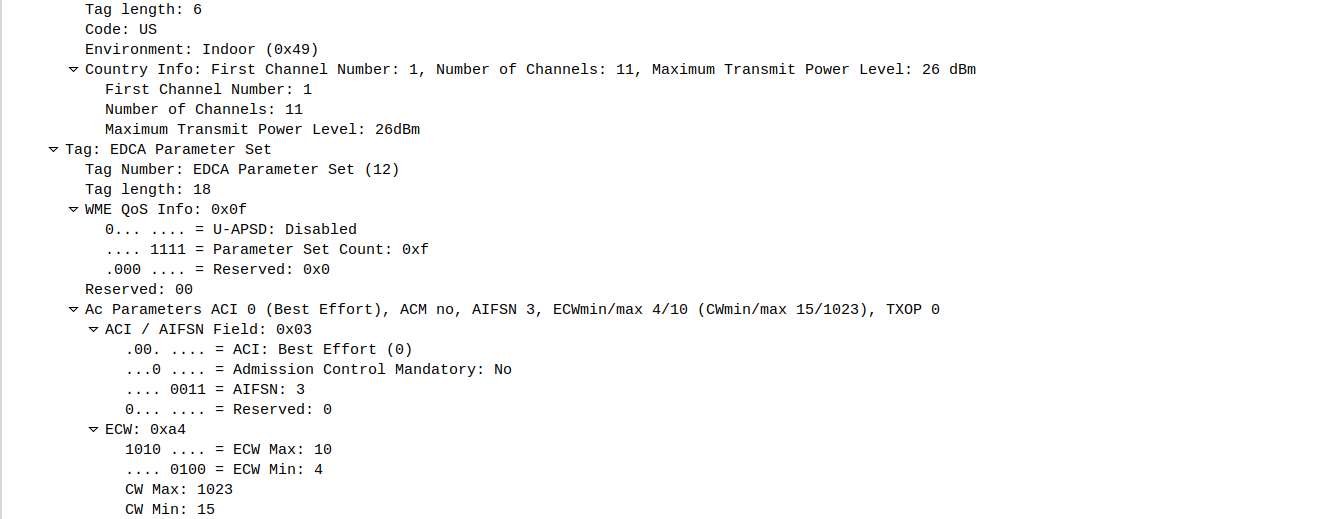
\includegraphics[scale=0.3]{WLAN/correcto7.png}
\end{center}
\begin{center}
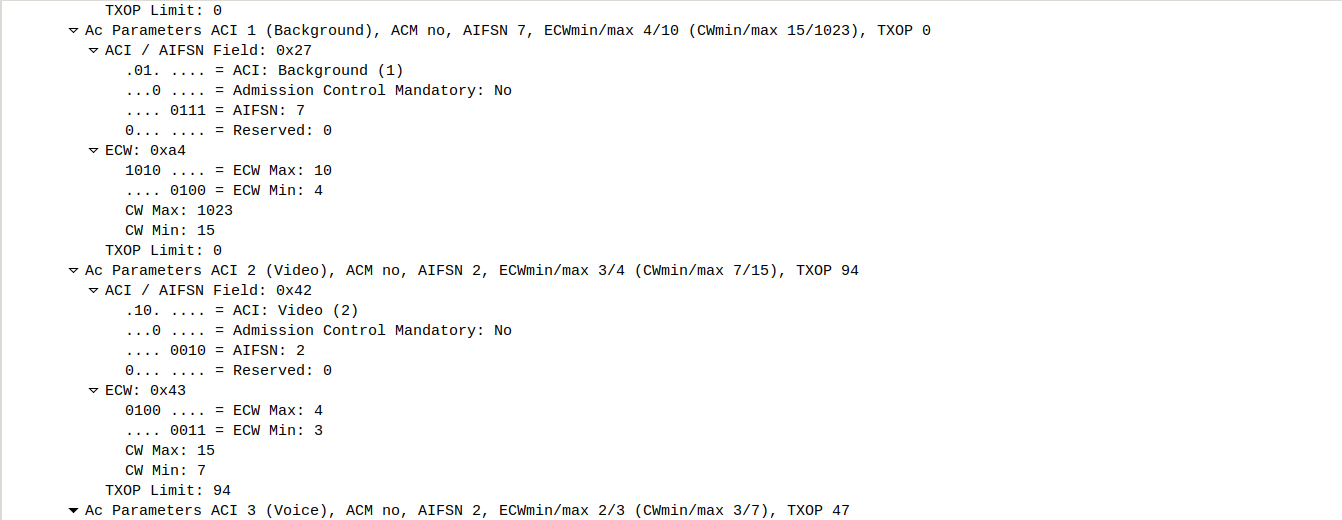
\includegraphics[scale=0.3]{WLAN/correcto8.png}
\end{center}
\begin{center}
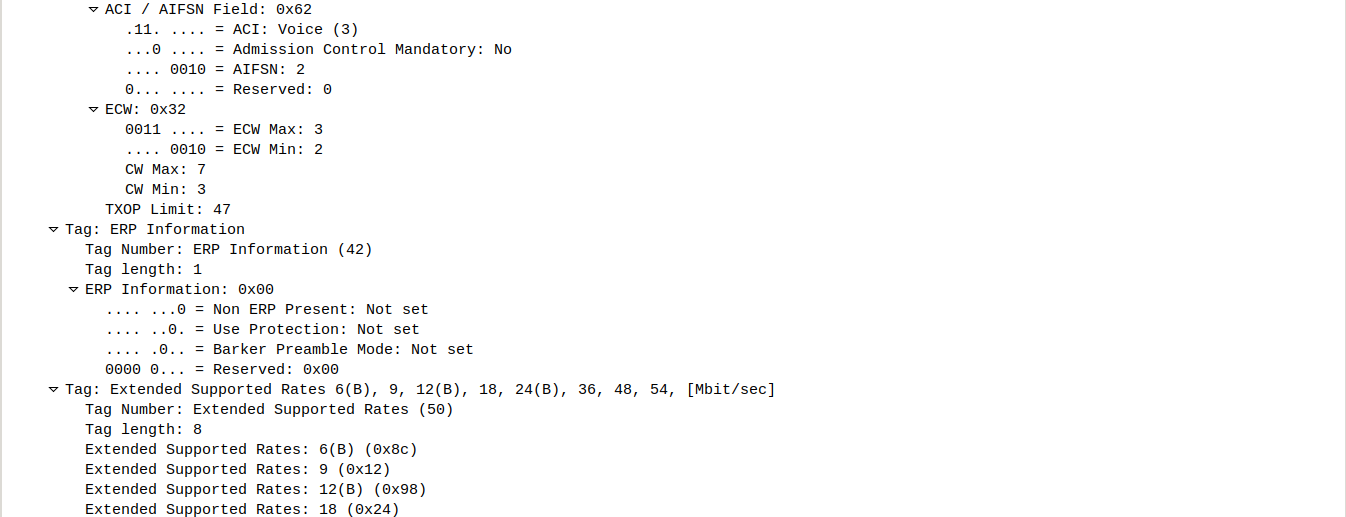
\includegraphics[scale=0.3]{WLAN/correcto9.png}
\end{center}
\begin{center}
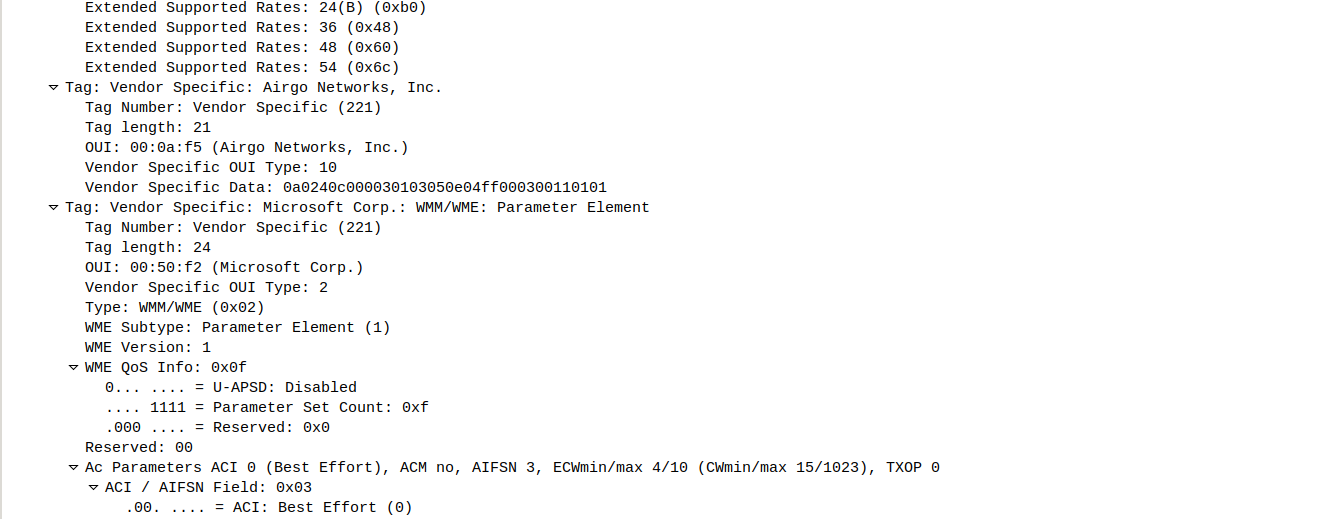
\includegraphics[scale=0.3]{WLAN/correcto10.png}
\end{center}
\begin{center}
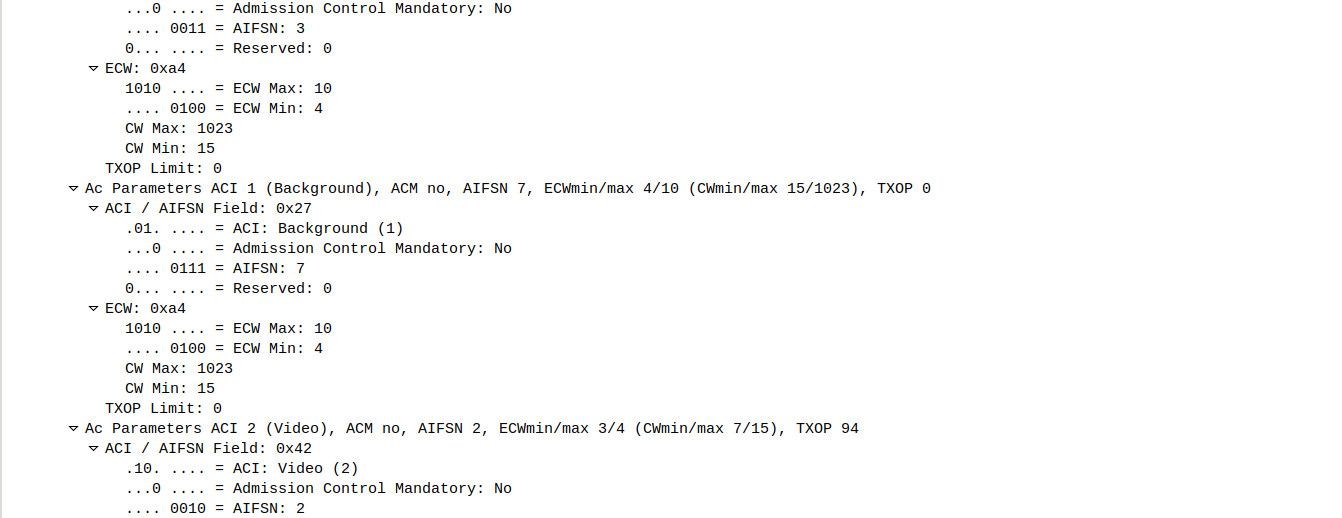
\includegraphics[scale=0.3]{WLAN/correcto11.png}
\end{center}
\begin{center}
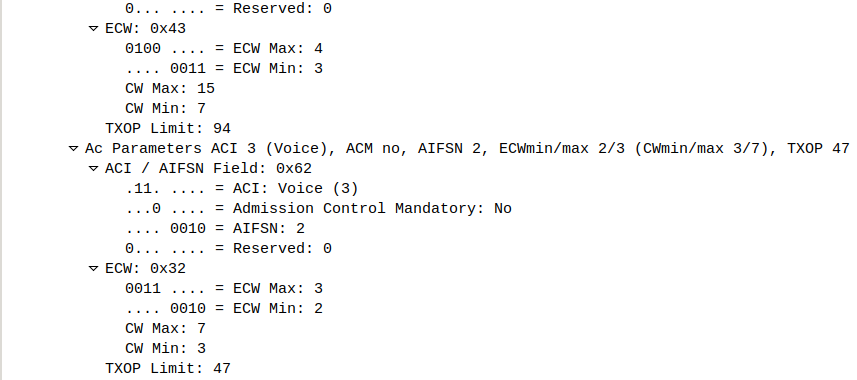
\includegraphics[scale=0.3]{WLAN/correcto12.png}
\end{center}

\textbf{Trama Beacon incorrecta}

\begin{center}
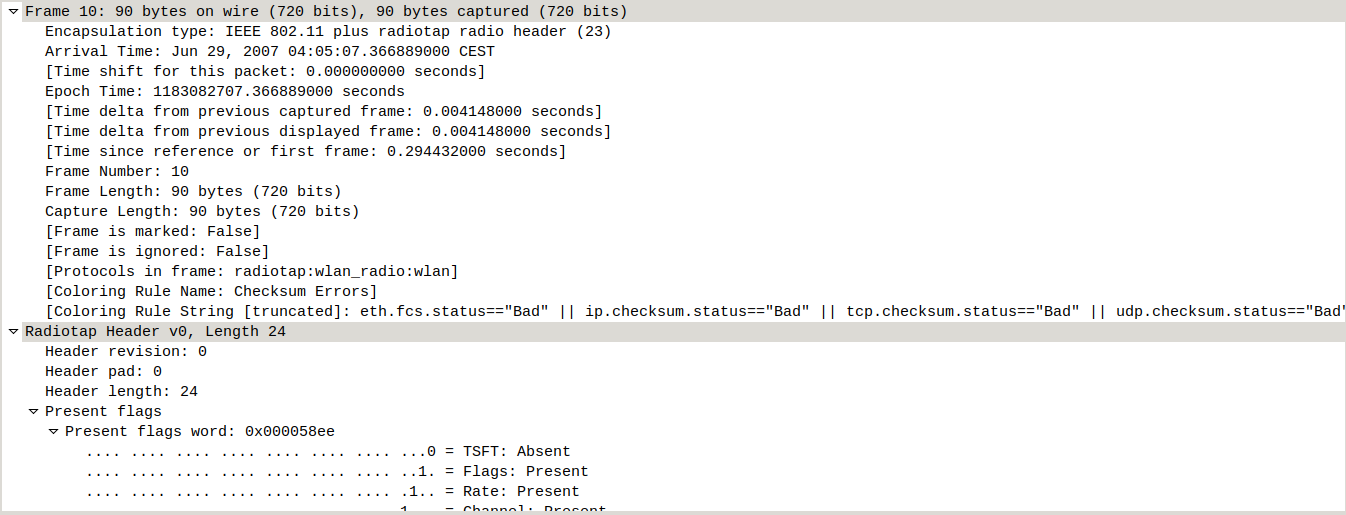
\includegraphics[scale=0.3]{WLAN/inco1.png}
\end{center}
\begin{center}
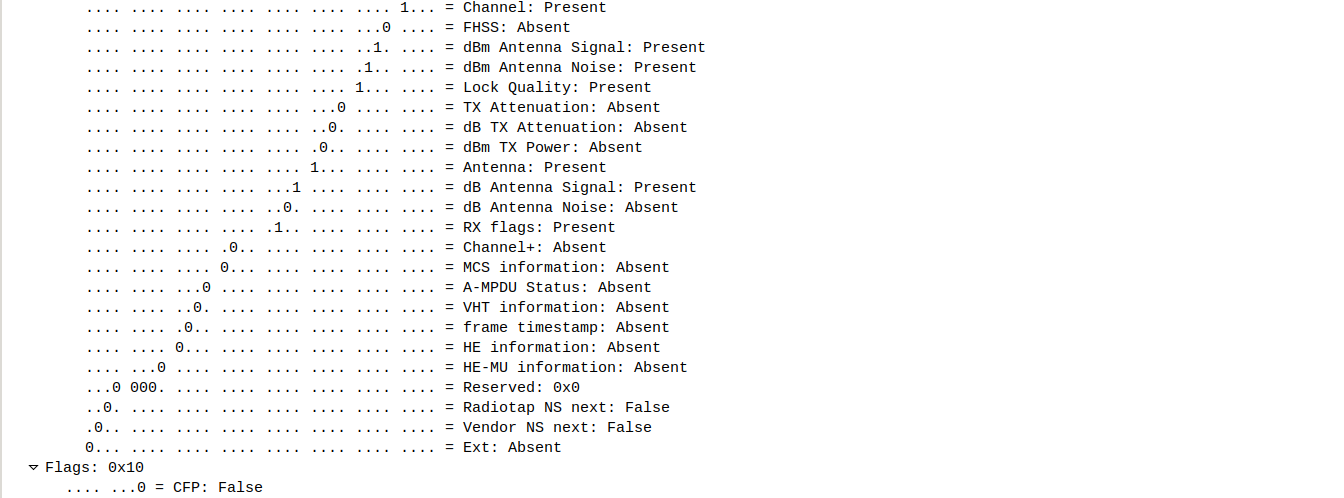
\includegraphics[scale=0.3]{WLAN/inco2.png}
\end{center}
\begin{center}
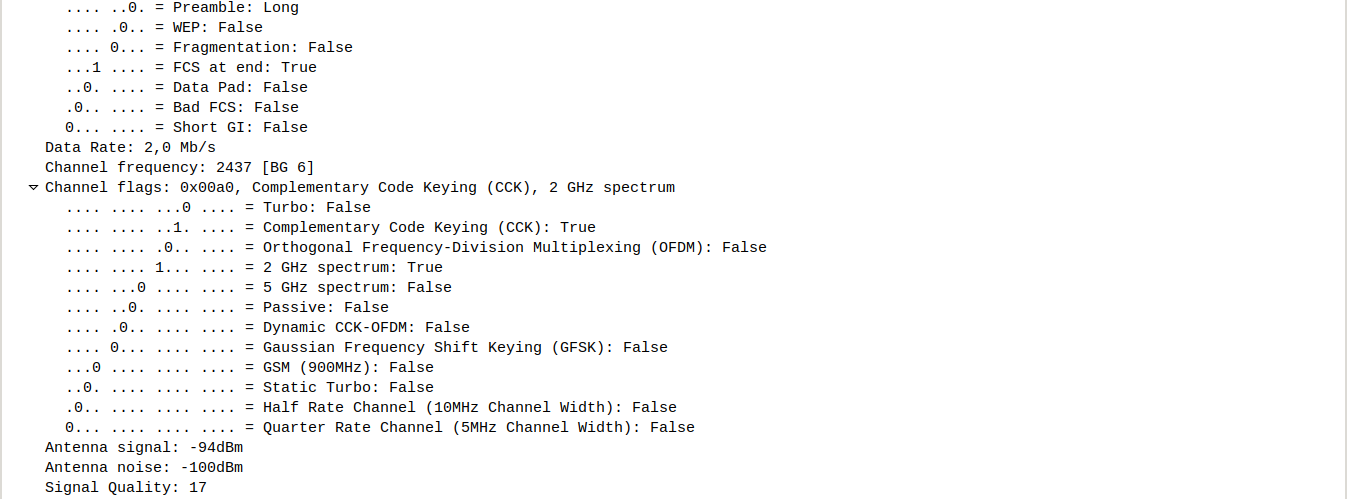
\includegraphics[scale=0.3]{WLAN/inco3.png}
\end{center}
\begin{center}
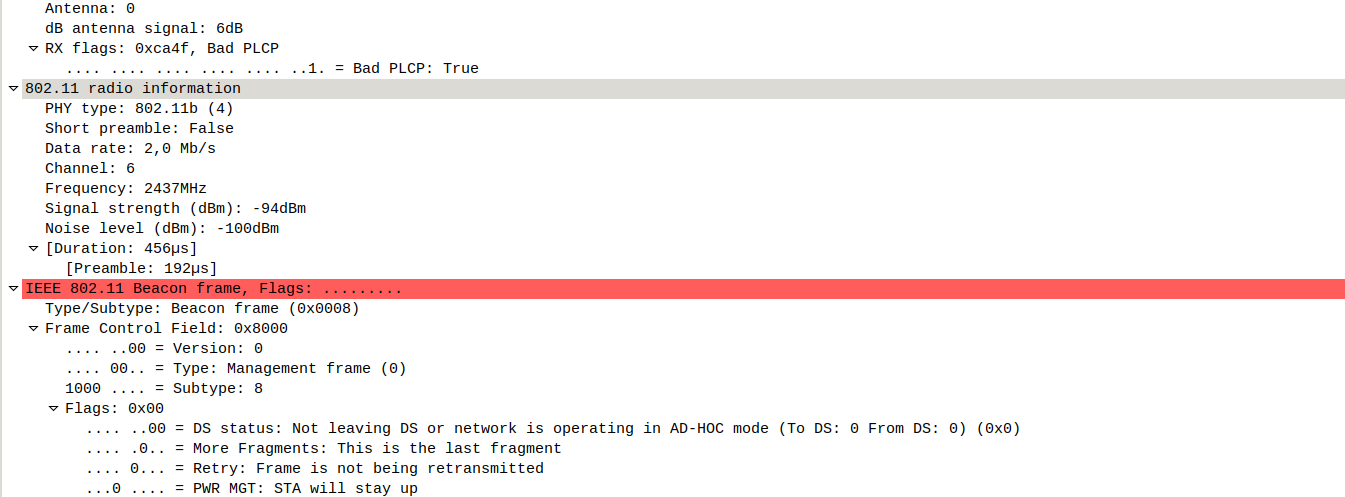
\includegraphics[scale=0.3]{WLAN/inco4.png}
\end{center}
\begin{center}
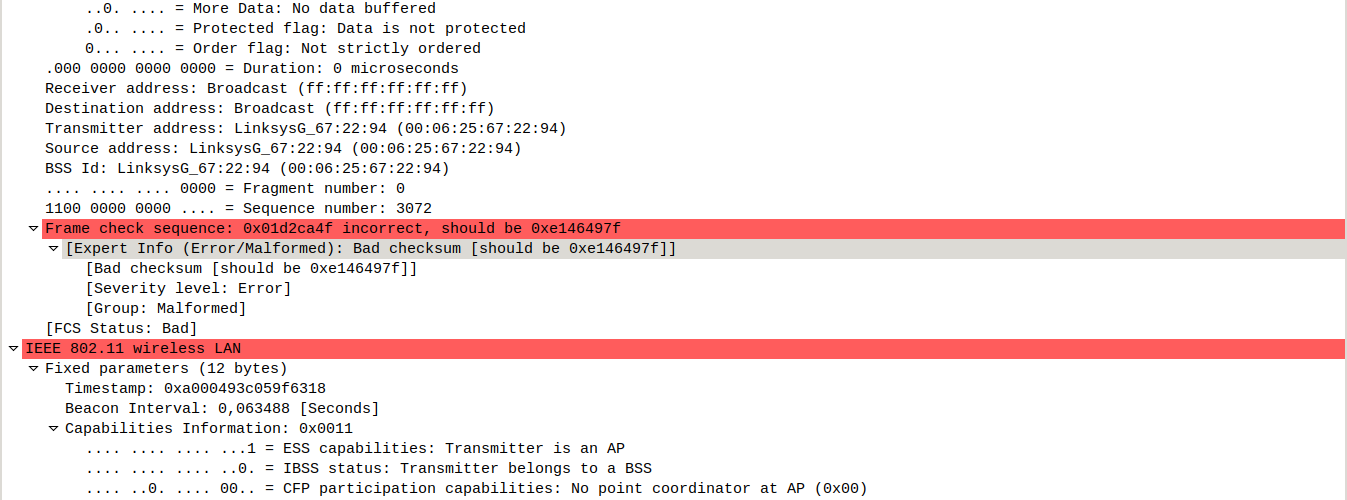
\includegraphics[scale=0.3]{WLAN/inco5.png}
\end{center}
\begin{center}
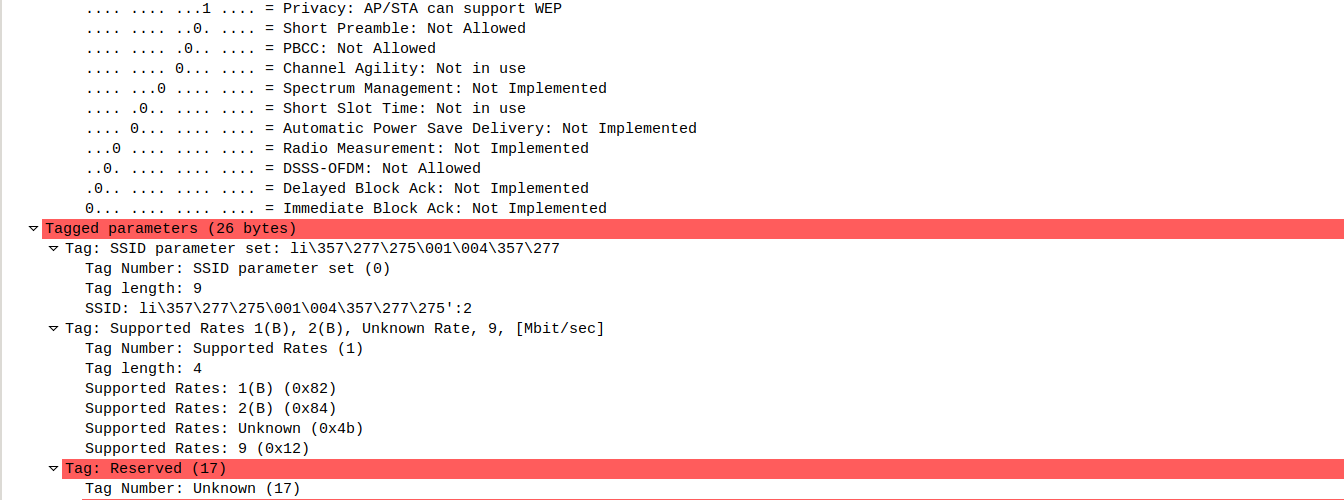
\includegraphics[scale=0.3]{WLAN/inco6.png}
\end{center}
\begin{center}
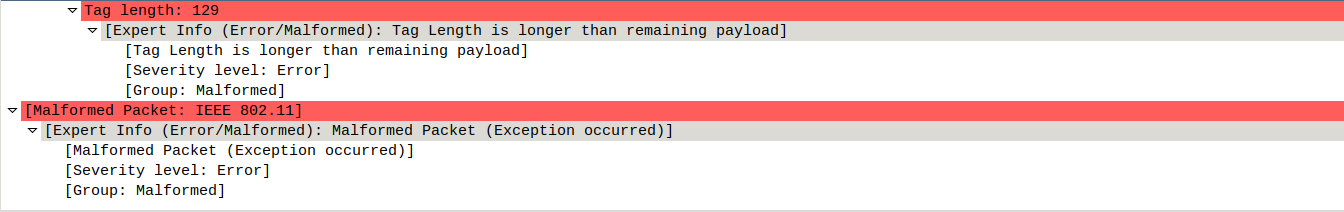
\includegraphics[scale=0.3]{WLAN/inco7.png}
\end{center}

\section{Cuestión 2}

\textbf{En la captura, ¿hay alguna estación que realice un escaneo activo? ¿Hay APs que
respondan? ¿Qué tipos de tramas son? (Consulta e indica el valor de campo tipo)}

Sí, se comprueban en las tramas Probe Request para las que escanean activamente y con las tramas Probe Response para las que responden a estos escaneos. Los tipos de tramas son 0 en ambos casos.

\begin{center}
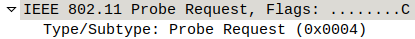
\includegraphics[scale=0.4]{WLAN/req.png}
\end{center}
\begin{center}
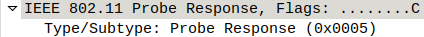
\includegraphics[scale=0.4]{WLAN/res.png}
\end{center}

\subsection{WLAN\_802\_11}

Las estaciones que escanean son las que se ven en las capturas, y solo una responde, 30 Munroe St.

\begin{center}
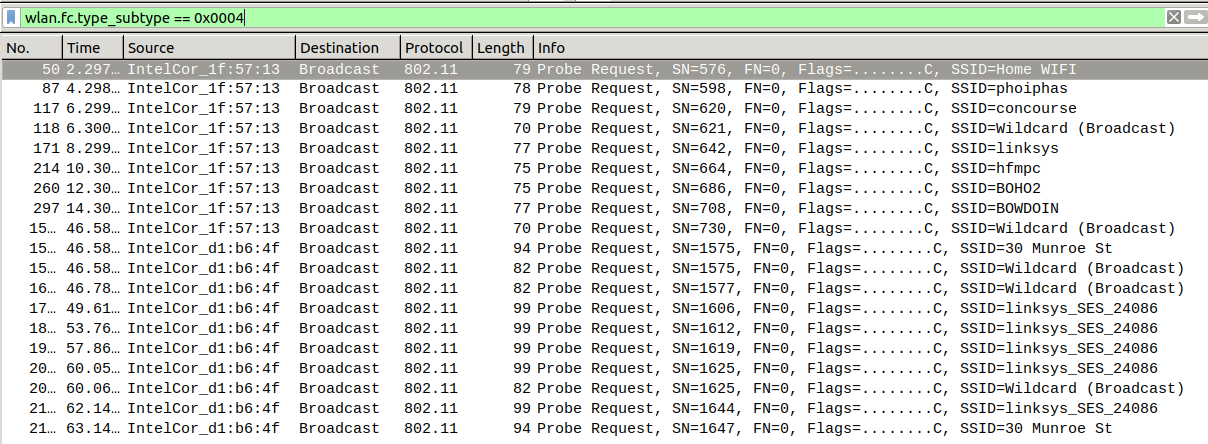
\includegraphics[scale=0.3]{WLAN/probreq.png}
\end{center}
\begin{center}
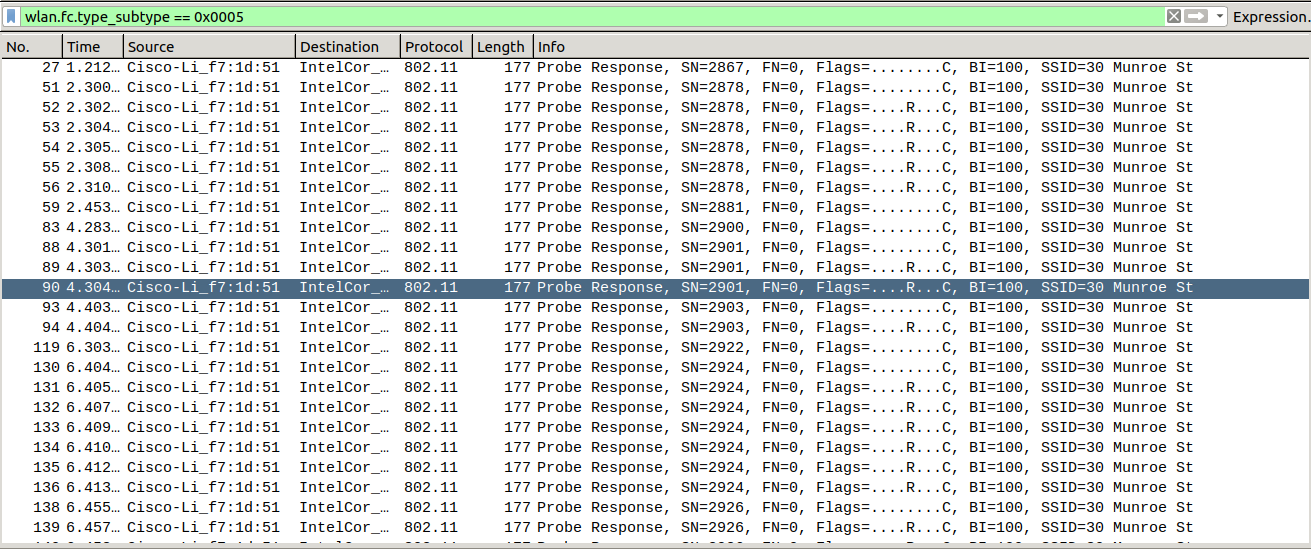
\includegraphics[scale=0.3]{WLAN/probres.png}
\end{center}

\subsection{WLAN\_802\_11LOCAL}

Las estaciones que escanean son las que se ven en las capturas. Para obtener las que responden, realizamos el mismo procedimiento de la primera cuestión, y son:

\begin{itemize}
\item alumnos
\item eduroam
\item WifiUma
\item GISUM\_W1
\item pdi
\item pas
\item NEO
\item ICB\-Wifi
\end{itemize}

\begin{center}
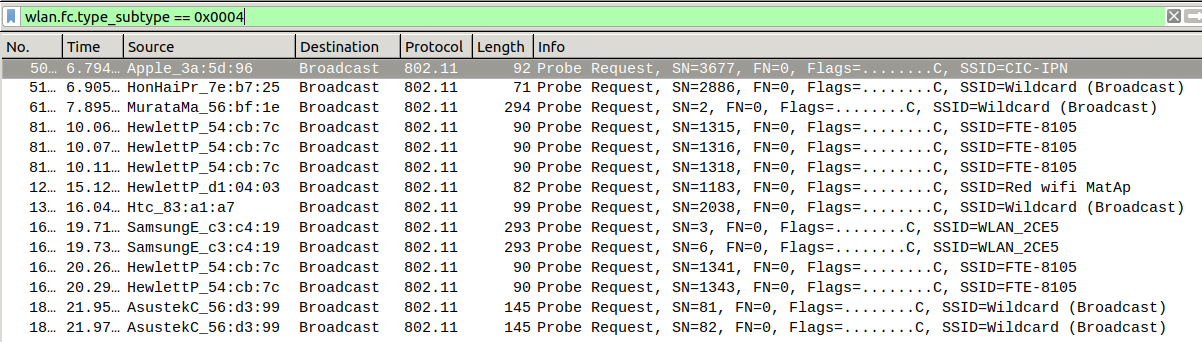
\includegraphics[scale=0.3]{WLAN/probreqlocal.png}
\end{center}
\begin{center}
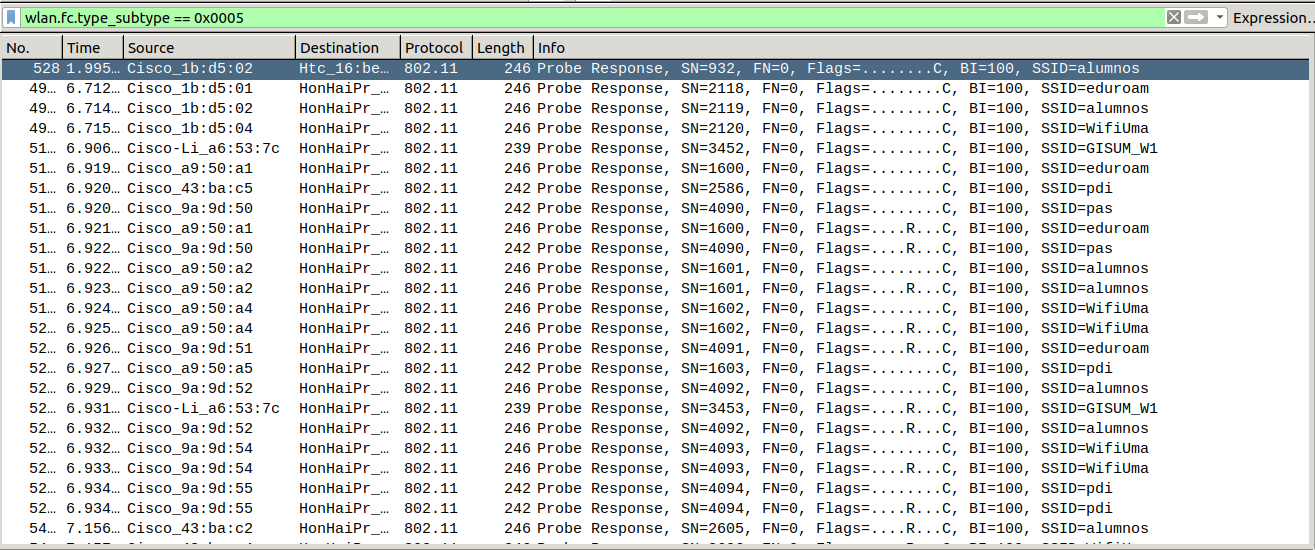
\includegraphics[scale=0.3]{WLAN/probreslocal.png}
\end{center}


\section{Ejercicio 2}

\textbf{Localiza en la captura alguna trama de petición activo y la respuesta
correspondiente. Muestra la estructura y contenido de ambas tramas.}

\begin{center}

\includegraphics[scale=0.3]{WLAN/probes.png}
\end{center}

\textbf{\underline{Probe Request}}

\begin{center}
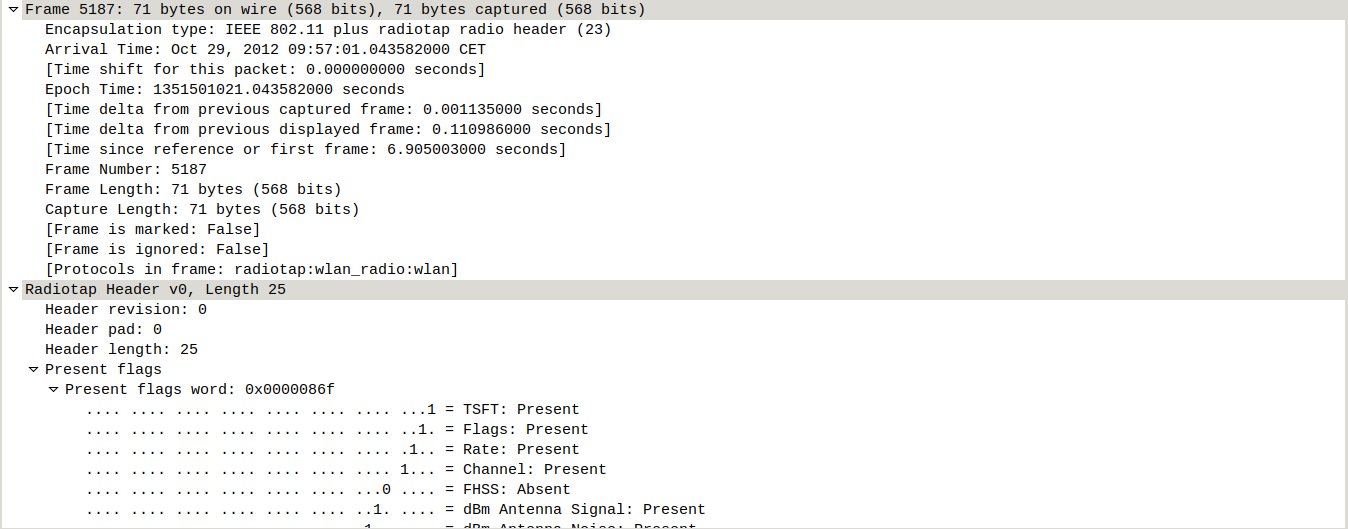
\includegraphics[scale=0.3]{WLAN/probreq1.png}
\end{center}
\begin{center}
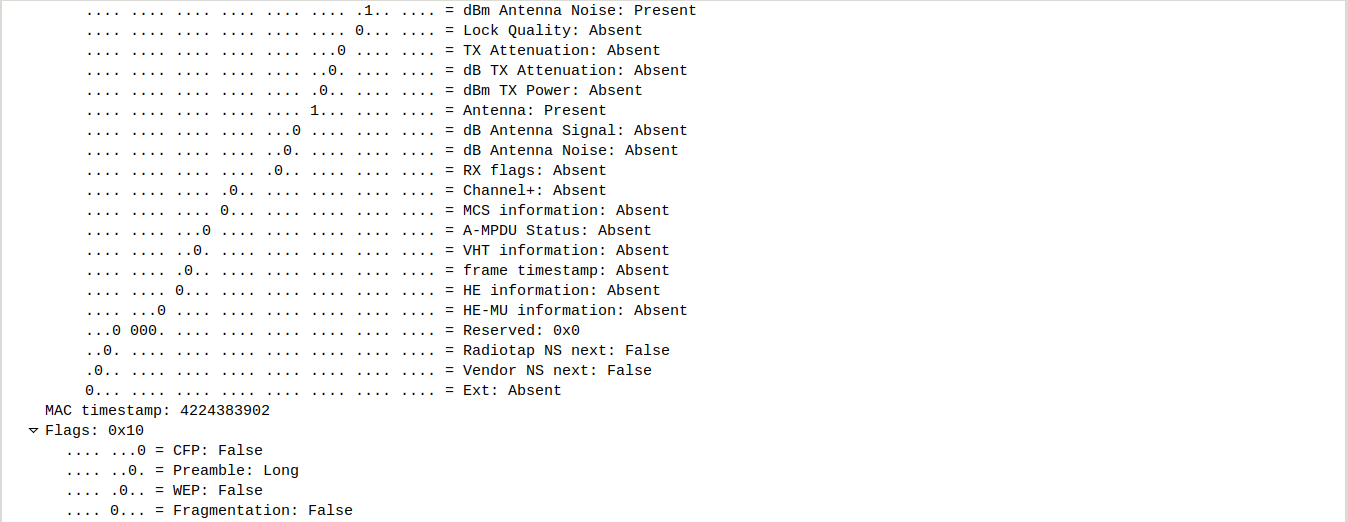
\includegraphics[scale=0.3]{WLAN/probreq2.png}
\end{center}
\begin{center}
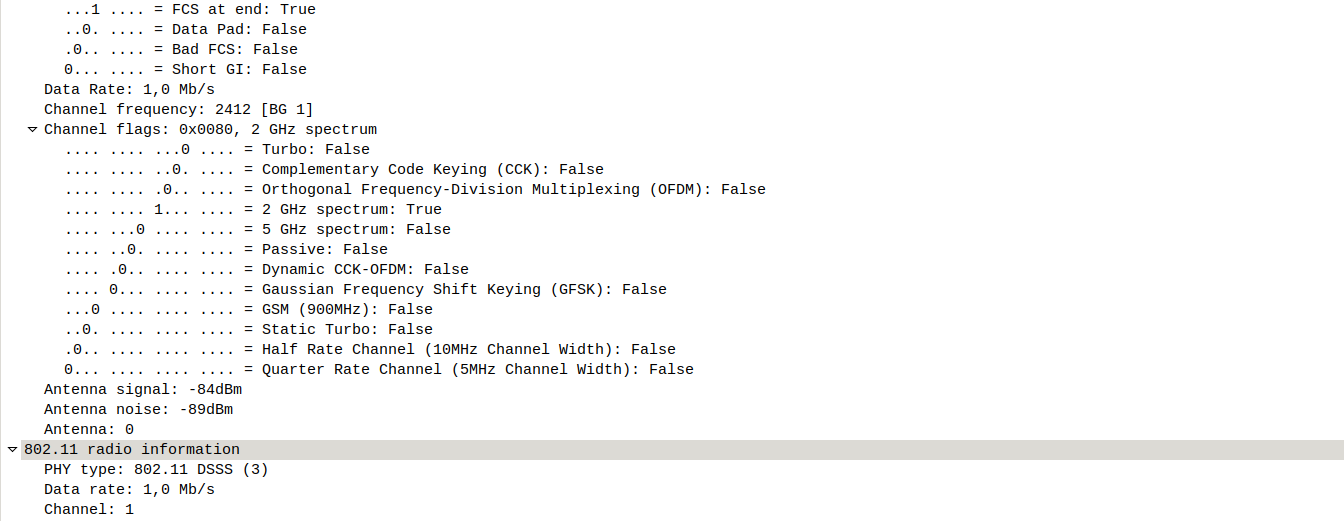
\includegraphics[scale=0.3]{WLAN/probreq3.png}
\end{center}
\begin{center}
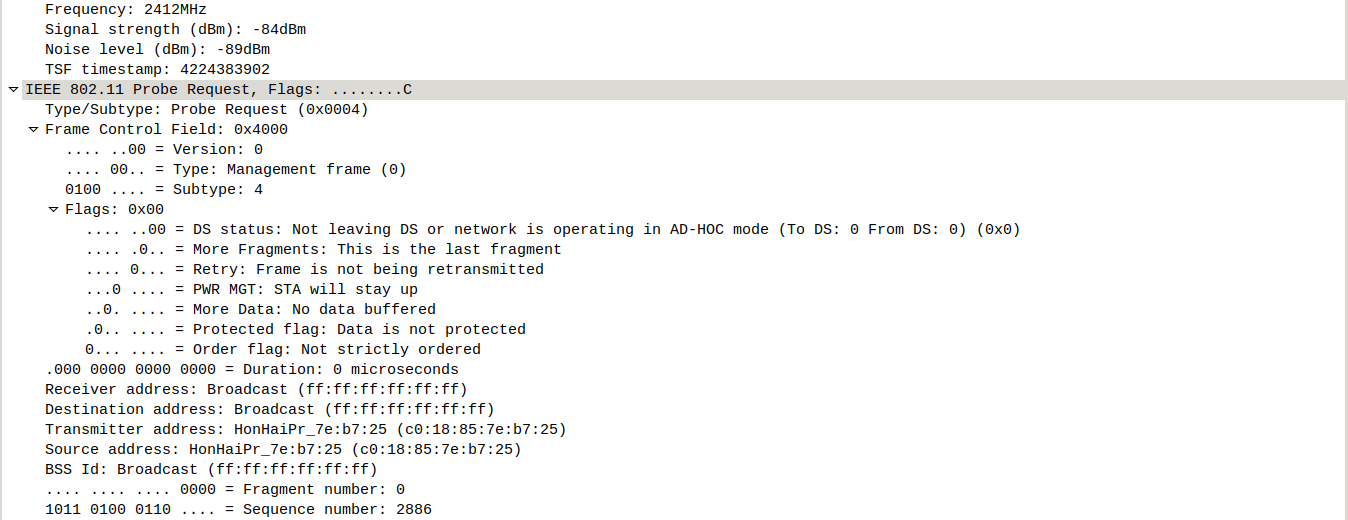
\includegraphics[scale=0.3]{WLAN/probreq4.png}
\end{center}
\begin{center}
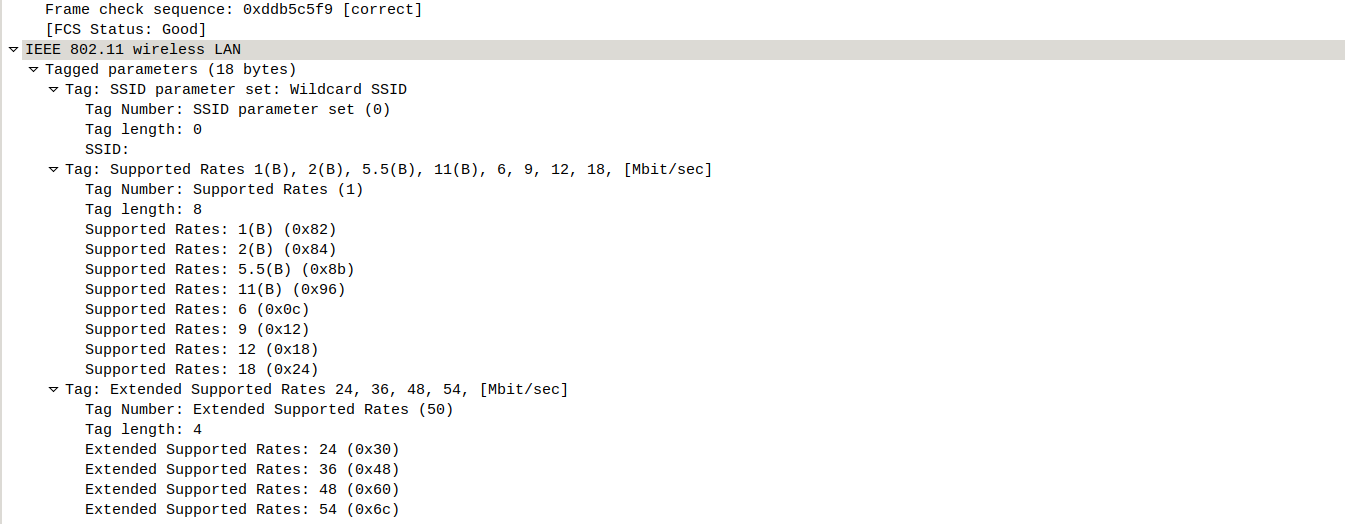
\includegraphics[scale=0.3]{WLAN/probreq5.png}
\end{center}
\begin{center}
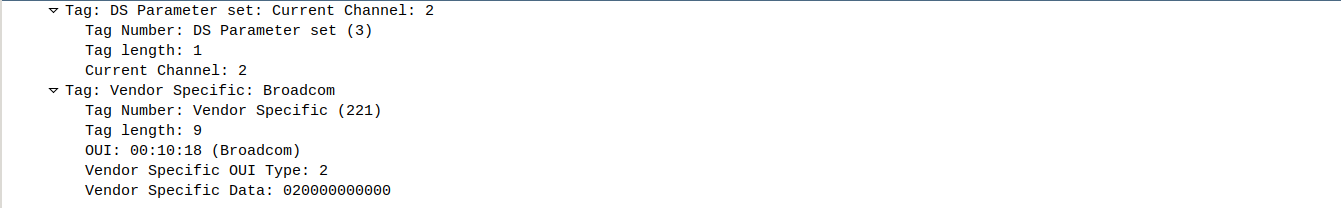
\includegraphics[scale=0.3]{WLAN/probreq6.png}
\end{center}

\textbf{\underline{Probe Response}}

\begin{center}
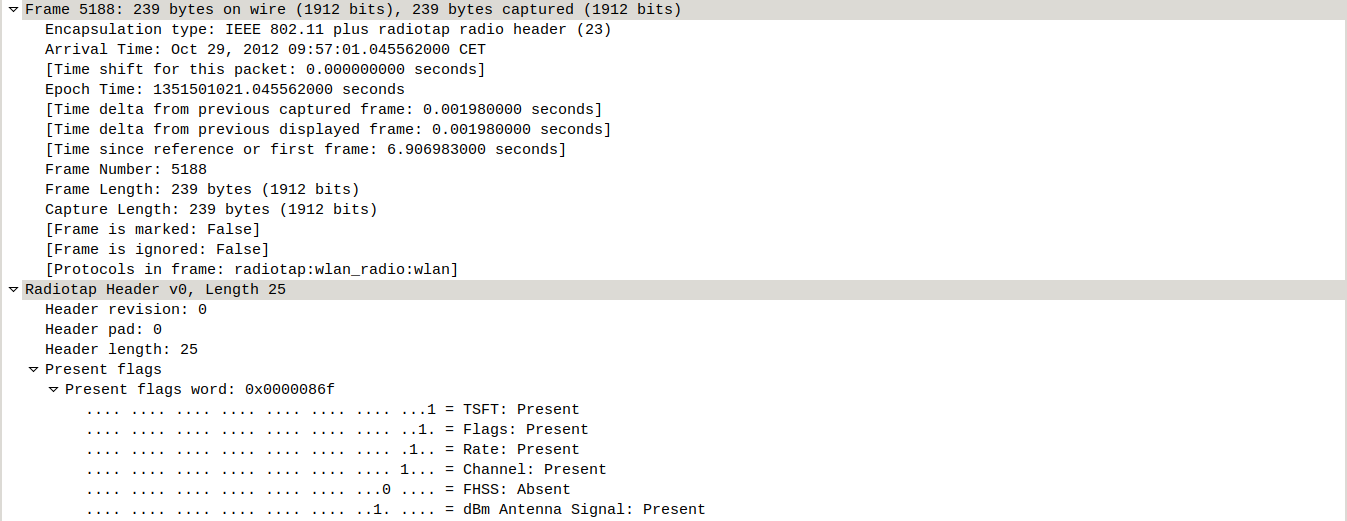
\includegraphics[scale=0.3]{WLAN/probres1.png}
\end{center}
\begin{center}
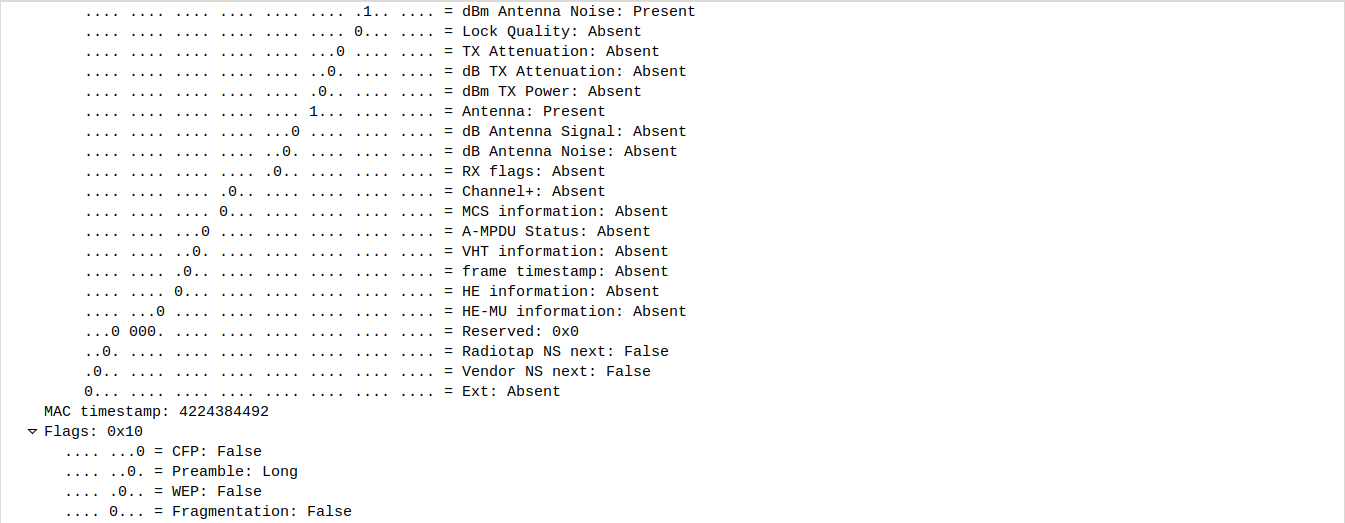
\includegraphics[scale=0.3]{WLAN/probres2.png}
\end{center}
\begin{center}
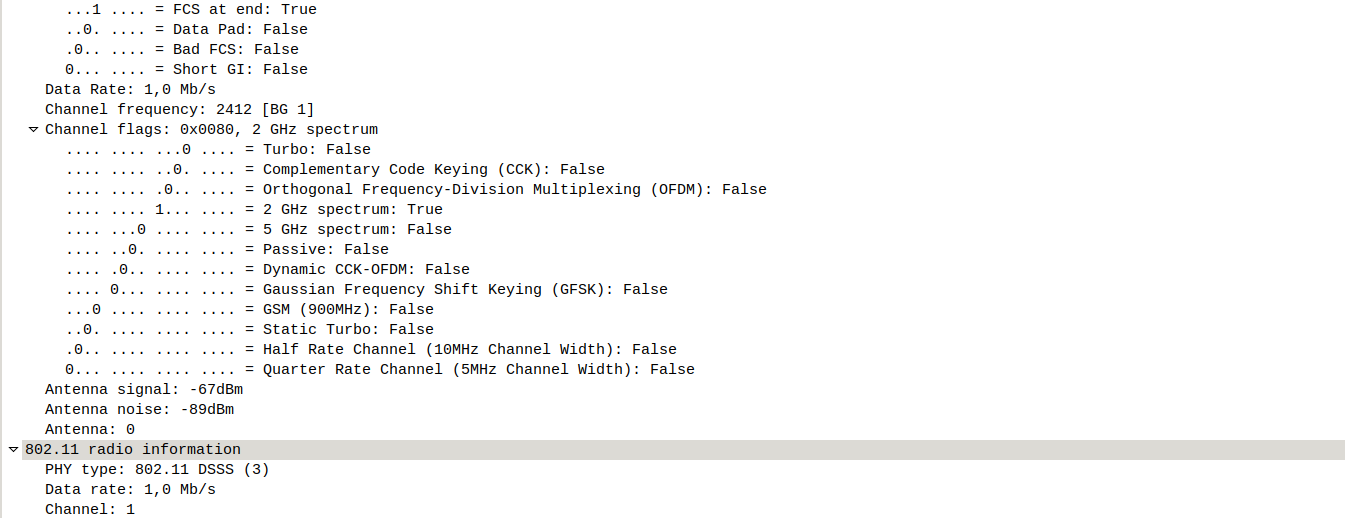
\includegraphics[scale=0.3]{WLAN/probres3.png}
\end{center}
\begin{center}
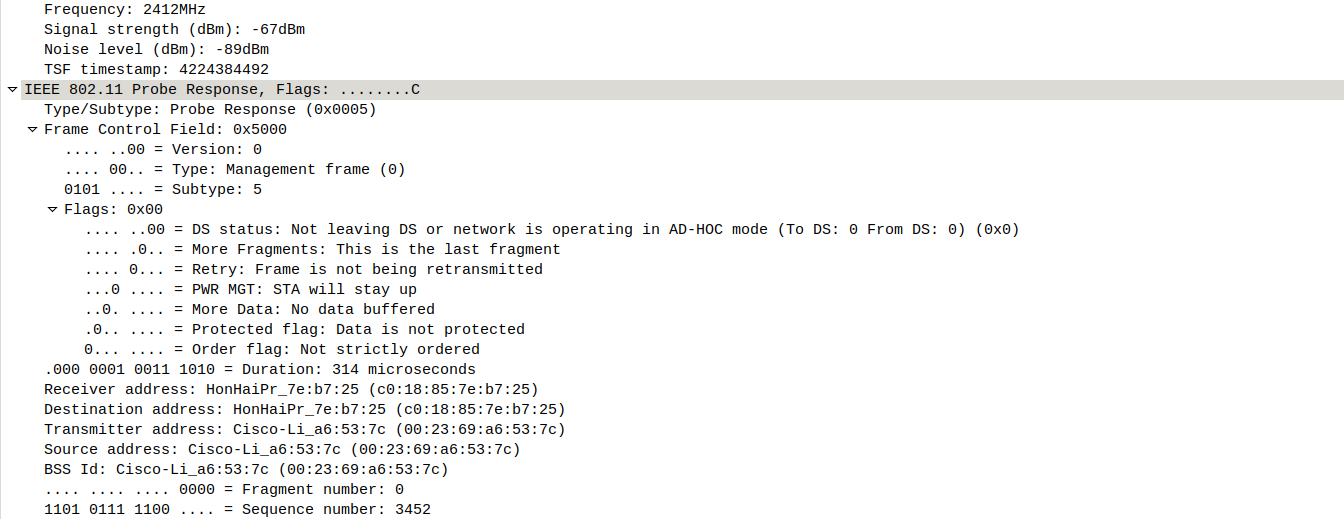
\includegraphics[scale=0.3]{WLAN/probres4.png}
\end{center}
\begin{center}
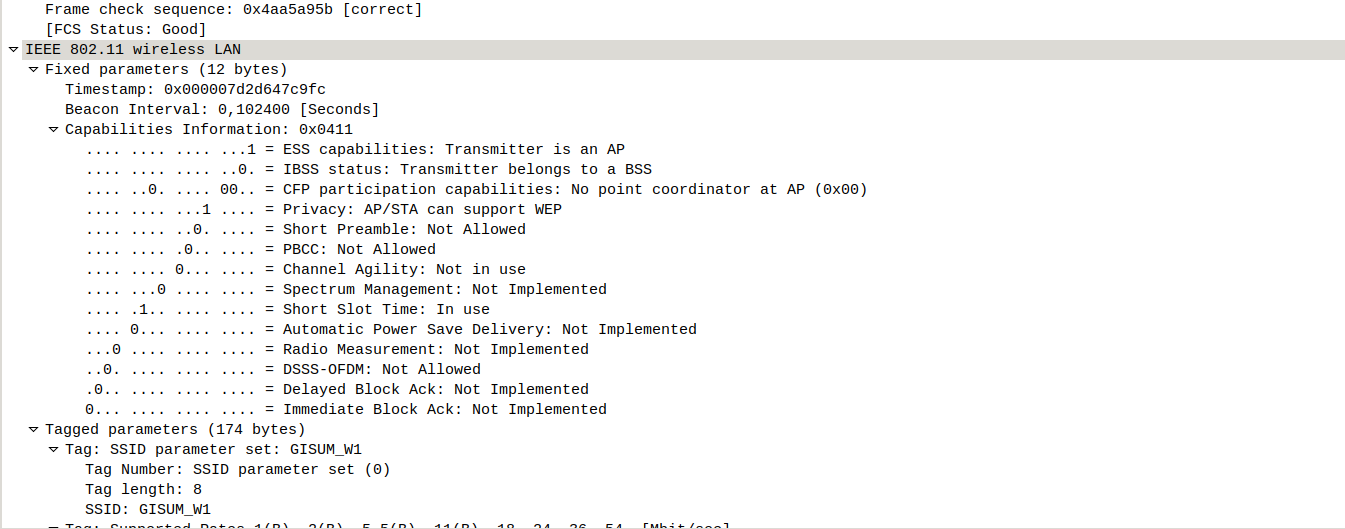
\includegraphics[scale=0.3]{WLAN/probres5.png}
\end{center}
\begin{center}
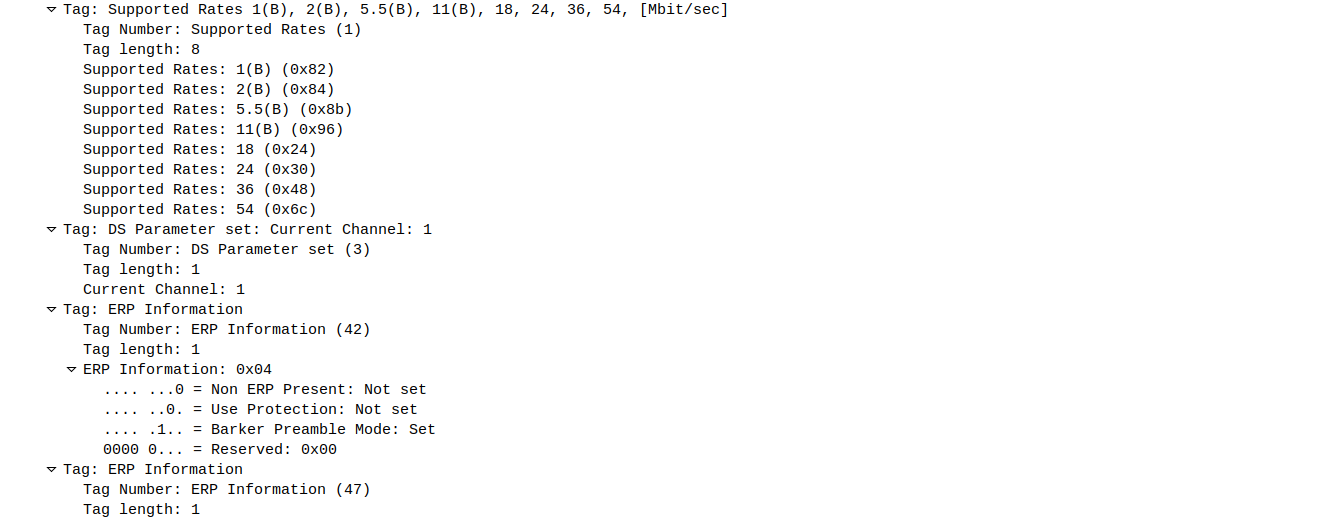
\includegraphics[scale=0.3]{WLAN/probres6.png}
\end{center}
\begin{center}
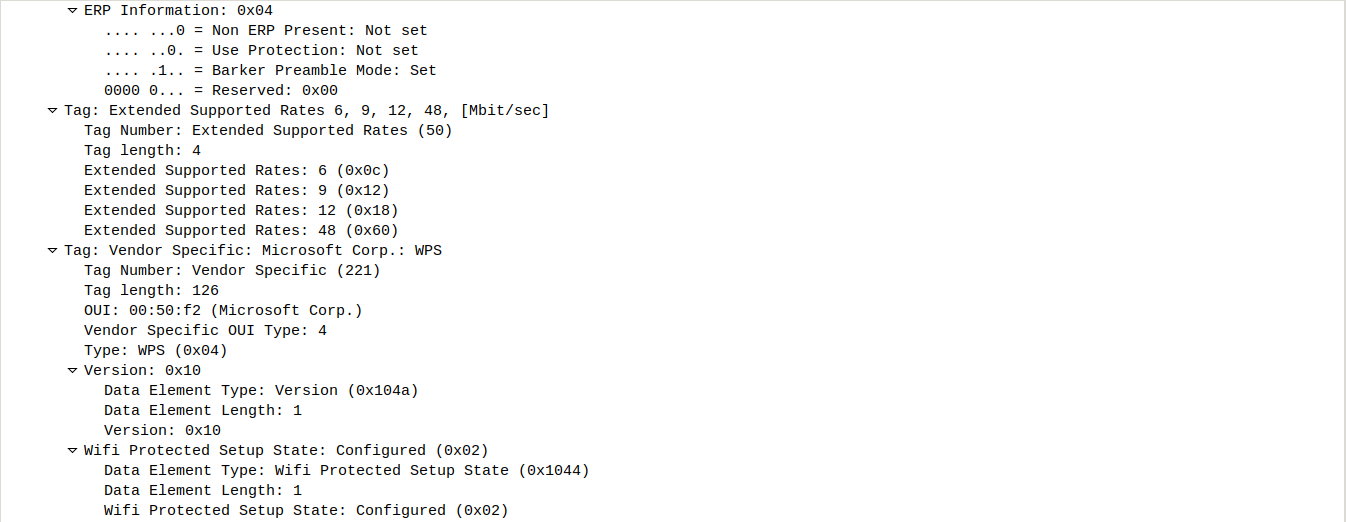
\includegraphics[scale=0.3]{WLAN/probres7.png}
\end{center}
\begin{center}
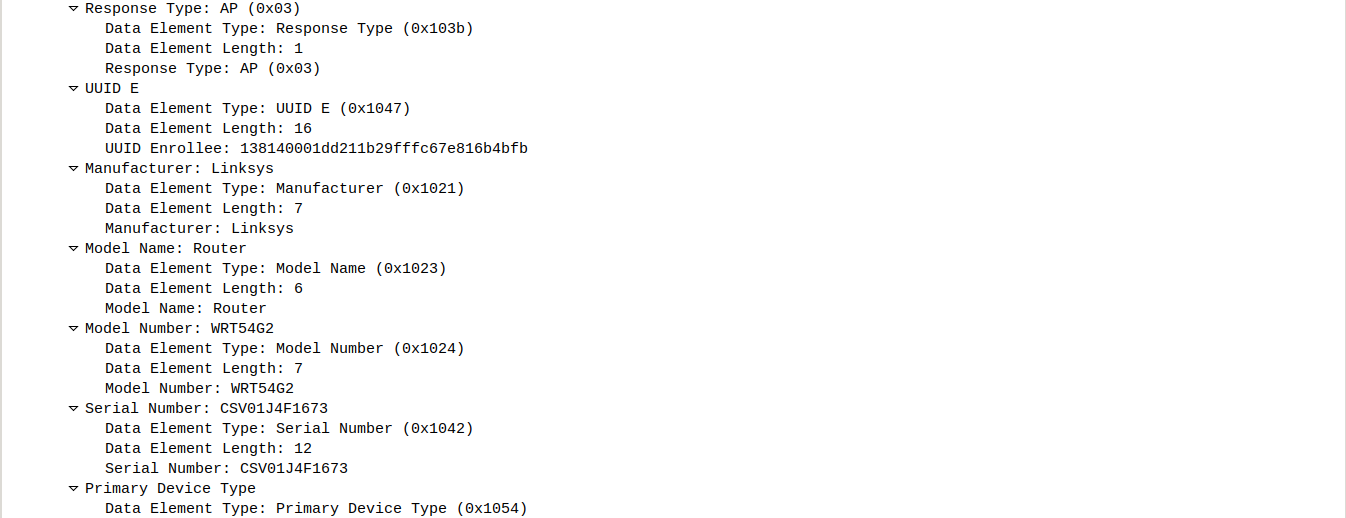
\includegraphics[scale=0.3]{WLAN/probres8.png}
\end{center}
\begin{center}
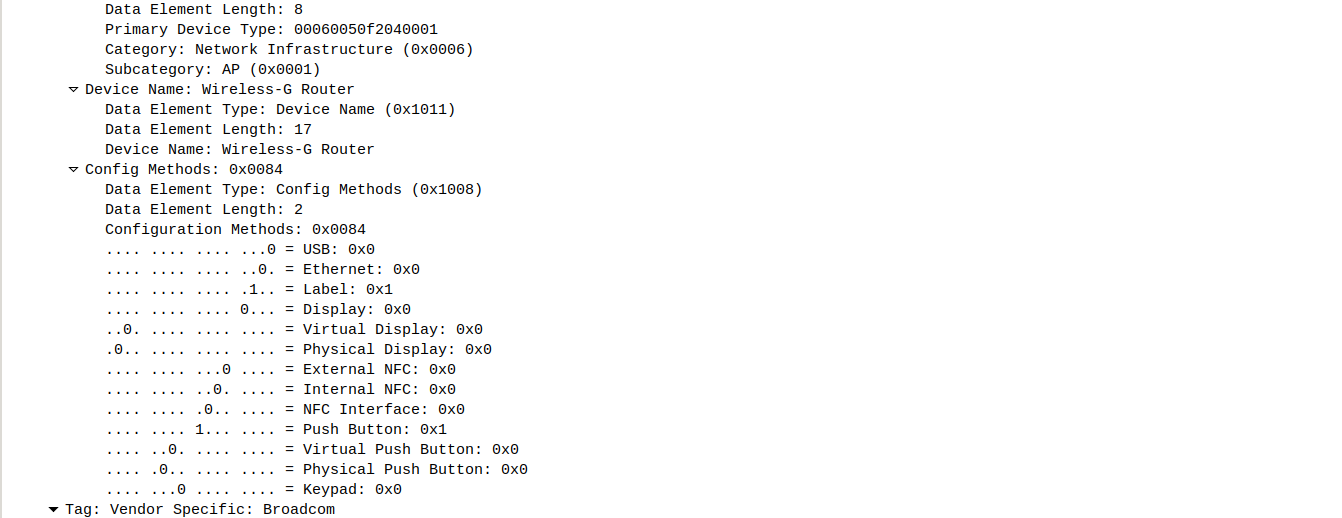
\includegraphics[scale=0.3]{WLAN/probres9.png}
\end{center}
\begin{center}
\includegraphics[scale=0.3]{WLAN/probres10.png}
\end{center}


\section{Cuestión 3}

\textbf{Localiza en la captura alguna petición de asociación. ¿Qué información incluye?
Localiza en la captura alguna respuesta de asociación ¿Qué información incluye? ¿Qué tipos de
tramas con? (valor de campo tipo)}

\begin{center}
\includegraphics[scale=0.3]{WLAN/assreq.png}
\end{center}
\begin{center}
\includegraphics[scale=0.4]{WLAN/assreqt.png}
\end{center}

\begin{center}
\includegraphics[scale=0.3]{WLAN/assres.png}
\end{center}
\begin{center}
\includegraphics[scale=0.4]{WLAN/assrest.png}
\end{center}

\section{Ejercicio 3}

\textbf{Localiza en la captura alguna trama de petición de asociación y la respuesta
correspondiente. Muestra la estructura y contenido de ambas tramas}

\textbf{\underline{Petición de asociación}}

\begin{center}
\includegraphics[scale=0.3]{WLAN/assreq1.png}
\end{center}
\begin{center}
\includegraphics[scale=0.3]{WLAN/assreq2.png}
\end{center}
\begin{center}
\includegraphics[scale=0.3]{WLAN/assreq3.png}
\end{center}
\begin{center}
\includegraphics[scale=0.3]{WLAN/assreq4.png}
\end{center}
\begin{center}
\includegraphics[scale=0.3]{WLAN/assreq5.png}
\end{center}
\begin{center}
\includegraphics[scale=0.3]{WLAN/assreq6.png}
\end{center}
\begin{center}
\includegraphics[scale=0.3]{WLAN/assreq7.png}
\end{center}

\textbf{\underline{Respuesta}}

\begin{center}
\includegraphics[scale=0.3]{WLAN/assres1.png}
\end{center}
\begin{center}
\includegraphics[scale=0.3]{WLAN/assres2.png}
\end{center}
\begin{center}
\includegraphics[scale=0.3]{WLAN/assres3.png}
\end{center}
\begin{center}
\includegraphics[scale=0.3]{WLAN/assres4.png}
\end{center}
\begin{center}
\includegraphics[scale=0.3]{WLAN/assres5.png}
\end{center}
\begin{center}
\includegraphics[scale=0.3]{WLAN/assres6.png}
\end{center}
\begin{center}
\includegraphics[scale=0.3]{WLAN/assres7.png}
\end{center}
\begin{center}
\includegraphics[scale=0.3]{WLAN/assres8.png}
\end{center}

\section{Cuestión 4}

\textbf{¿Cual de estos dos escenarios correspondería con un escaneado pasivo y con uno
activo? ¿Por qué?}

\begin{center}
\includegraphics[scale=0.4]{WLAN/c4.png}
\end{center}

El escenario B, ya que hay comunicación directa entre los Puntos de Acceso sin necesidad de un intermediario.

\section{Cuestión 5}

\textbf{¿Cuántas tramas de datos diferentes observas en la captura? ¿Qué estaciones
participan de esta comunicación? ¿Hay comunicación directa entre estaciones o siempre
interviene un punto de acceso?}

\begin{center}
\includegraphics[scale=0.3]{WLAN/lista.png}
\end{center}

Hay bastantes subtipos de tramas de datos. Los que más se repiten son:

\begin{itemize}
\item Standard query
\item QoS Null Function (No data)
\item Null Function (No data)
\item ACK
\item SYN-ACK
\item PSH-ACK
\end{itemize}

\begin{center}
\includegraphics[scale=0.3]{WLAN/BSSID.png}
\end{center}

Las estaciones que participan son las de la imagen anterior. Siempre interviene un Punto de Acceso en la comunicación, como es normal en este tipo de comunicaciones.

\section{Ejercicio 4}

\textbf{Localiza en la captura alguna trama de datos y la confirmación correspondiente.
Muestra la estructura y contenido de ambas tramas.}

\begin{center}
\includegraphics[scale=0.3]{WLAN/tramatcp.png}
\end{center}

\textbf{\underline{Trama de datos}}

\begin{center}
\includegraphics[scale=0.3]{WLAN/tcpres1.png}
\end{center}
\begin{center}
\includegraphics[scale=0.3]{WLAN/tcpres2.png}
\end{center}
\begin{center}
\includegraphics[scale=0.3]{WLAN/tcpres3.png}
\end{center}
\begin{center}
\includegraphics[scale=0.3]{WLAN/tcpres5.png}
\end{center}
\begin{center}
\includegraphics[scale=0.3]{WLAN/tcpres6.png}
\end{center}
\begin{center}
\includegraphics[scale=0.3]{WLAN/tcpres7.png}
\end{center}
\begin{center}
\includegraphics[scale=0.3]{WLAN/tcpres8.png}
\end{center}
\begin{center}
\includegraphics[scale=0.3]{WLAN/tcpres9.png}
\end{center}

\textbf{\underline{Confirmación}}

\begin{center}
\includegraphics[scale=0.3]{WLAN/tcpreq1.png}
\end{center}
\begin{center}
\includegraphics[scale=0.3]{WLAN/tcpreq2.png}
\end{center}
\begin{center}
\includegraphics[scale=0.3]{WLAN/tcpreq3.png}
\end{center}
\begin{center}
\includegraphics[scale=0.3]{WLAN/tcpreq4.png}
\end{center}
\begin{center}
\includegraphics[scale=0.3]{WLAN/tcpreq5.png}
\end{center}
\begin{center}
\includegraphics[scale=0.3]{WLAN/tcpreq6.png}
\end{center}
\begin{center}
\includegraphics[scale=0.3]{WLAN/tcpreq7.png}
\end{center}
\begin{center}
\includegraphics[scale=0.3]{WLAN/tcpreq8.png}
\end{center}

\section{Ejercicio 5}

\textbf{Localiza en la captura alguna trama de datos NULL Muestra la estructura y
contenido de esta trama. ¿Qué la diferencia de las tramas de datos normales? ¿Para qué sirve?}

\begin{center}
\includegraphics[scale=0.3]{WLAN/nf.png}
\end{center}

La principal diferencia es la ausencia del payload en la trama de datos y del campo de cuerpo. Se usa para mantener activo el canal de asociación, aprovechándose de su ligereza de su cabecera para un mayor ahorro energético.

\begin{center}
\includegraphics[scale=0.3]{WLAN/nf1.png}
\end{center}
\begin{center}
\includegraphics[scale=0.3]{WLAN/nf2.png}
\end{center}
\begin{center}
\includegraphics[scale=0.3]{WLAN/nf3.png}
\end{center}
\begin{center}
\includegraphics[scale=0.3]{WLAN/nf4.png}
\end{center}
\begin{center}
\includegraphics[scale=0.3]{WLAN/nf5.png}
\end{center}


\section{Cuestión 6}

\textbf{Encuentra la trama que contenga el segmento TCP SYN de la primera sesión TCP
(que descarga alice.txt). Muestra su contenido.}

\begin{center}
\includegraphics[scale=0.3]{WLAN/flags.png}
\end{center}
\begin{center}
\includegraphics[scale=0.3]{WLAN/packet.png}
\end{center}
\begin{center}
\includegraphics[scale=0.3]{WLAN/txt.png}
\end{center}

\subsection{6.a}

\textbf{¿Cuáles son las tres direcciones MAC de esta trama? ¿Cuál es la dirección MAC
correspondiente al host inalámbrico desde el que se hace la petición? (representación
hexadecimal) ¿Cuál la del punto de acceso? ¿y la del (primer) router?}

\begin{itemize}
\item \textbf{Dirección MAC del host:} 00:13:02:d1:b6:4f
\item \textbf{Punto de Acceso:} 00:16:b6:f7:1d:51
\item \textbf{Primer router:} 00:13:02:d1:b6:4f
\end{itemize}

\begin{center}
\includegraphics[scale=0.4]{WLAN/MAC.png}
\end{center}

\subsection{6.b}

\textbf{¿Cuáles es la dirección IP del host inalámbrico que envía este segmento? ¿y la dirección IP destino? ¿con que se corresponde esta dirección IP destino? (host, punto de acceso, router, o cualquier otro dispositivo de la red). Razona tu respuesta}

\begin{itemize}
\item \textbf{Host inalámbrico:} 192.168.1.109
\item \textbf{IP destino:} 128.119.245.12 (AP, ya quelos bits del mecanimo de direccionamiento están a 01)
\end{itemize}

\begin{center}
\includegraphics[scale=0.4]{WLAN/IP.png}
\end{center}

\section{Cuestión 7}

\textbf{Localiza las tramas RTS y CTS capturadas en el fichero Wireshar\_802\_11.pcap. ¿Es
posible que sólo haya tramas RTS o CTS? ¿Por qué?}

Tiene sentido que haya tramas RTS sin CTS, ya que se pueden efectuar peticiones sin que haya respuesta. Sin embargo, no lo tiene que sea al revés, ya que carece de sentido enviar una respuesta sin una petición.

\begin{center}
\includegraphics[scale=0.3]{WLAN/rts.png}
\end{center}
\begin{center}
\includegraphics[scale=0.3]{WLAN/cts.png}
\end{center}

\section{Cuestión 8}

\textbf{Localiza las tramas RTS y CTS capturadas en el fichero
Wireshar\_802\_11\_RTS\_CTS.pcap. ¿Qué información contiene estas tramas? ¿Para qué sirve
el valor NAV?}

El valor NAV (Network Allocation Vector) se usa para calcular el tiempo que el medio está siendo usado, y por lo tanto, saber cuándo enviar peticiones para usarlo y así reducir las colisiones de peticiones.

\textbf{\underline{RTS}}

\begin{center}
\includegraphics[scale=0.3]{WLAN/rts1.png}
\end{center}
\begin{center}
\includegraphics[scale=0.3]{WLAN/rts2.png}
\end{center}
\begin{center}
\includegraphics[scale=0.3]{WLAN/rts3.png}
\end{center}

\textbf{\underline{CTS}}

\begin{center}
\includegraphics[scale=0.3]{WLAN/cts1.png}
\end{center}
\begin{center}
\includegraphics[scale=0.3]{WLAN/cts2.png}
\end{center}
\begin{center}
\includegraphics[scale=0.3]{WLAN/cts3.png}
\end{center}

\end{document}